\section{Code actions}
\label{sec:codeact}

Native tool calls have a limit that \cref{sec:native} identified. A reply cannot loop or branch, so
every decision that depends on a tool result costs a turn, and every result passes through
the model context. Code actions remove this limit by making the model's action a program, which
the harness runs in an interpreter. The harness then no longer sees the individual operations, so
the dispatcher's checks and its per-call records no longer apply, and the budget on model calls no
longer bounds the work of a single action. This section shows what a design based on code actions
needs instead: a sandbox that confines writes, a record of each program's effects, limits that bound
its work, and care with instructions that arrive in observations. It ends with the second limit of
native calls, the cost of integrating every tool into every application separately, which leads to
Lecture~5.

\subsection{Code as the action}
\label{sec:codeact-action}

A \textbf{code action} is an action written as a program that the harness runs in an interpreter.
\textbf{CodeAct} is the approach in which the model's action is Python code, so that loops and
conditions run inside a single turn \citep{wang2024codeact}. With native calls, the model requests
one operation per call, and the dispatcher executes each call (\cref{sec:dispatcher}). With
CodeAct, the model writes the operations, and the control flow between them, as one program.

\Cref{lst:codeact-actions} shows the difference on an illustrative task: replace the comparison
\texttt{i <= n} with \texttt{i < n} in every Python file under \texttt{src}. The first action is a
\textbf{JSON action}, a tool call written as a JSON object that names the tool and its arguments.
It calls the \demoref{edit} tool of \msa{} once and changes one file. A native tool call is one kind
of JSON action. In the CodeAct study of \cref{sec:codeact-evidence}, JSON actions were written as
text in a format that the prompt described. The second action is a code action.
It loops over every Python file under \texttt{src} and rewrites each one. With JSON actions, the
same change needs one call per file, and further calls to find the files first, because a single
call cannot loop or branch.

\begin{lstlisting}[float=tbp, basicstyle=\ttfamily\footnotesize, columns=fixed, basewidth=0.525em, caption={Illustrative actions for the task of replacing \texttt{i <= n} with \texttt{i < n}. Above, a JSON action that edits one file. Below, a code action, sent as a shell command, that edits every matching file.}, label=lst:codeact-actions]
{"name": "edit",
 "arguments": {"path": "src/parse.py",
               "old": "i <= n", "new": "i < n"}}

python - <<'EOF'
import pathlib, re
for f in pathlib.Path("src").rglob("*.py"):
    s = f.read_text()
    f.write_text(re.sub(r"i <= n", "i < n", s))
EOF
\end{lstlisting}

The code action is a shell command. Its first line is shell syntax that passes the following
lines, up to \texttt{EOF}, to the Python interpreter as its input. A coding agent often sends its
code in this form, through a tool that runs shell commands. The Python interpreter of CodeAct
(\cref{sec:codeact-loop}) instead receives the Python lines directly. Both forms are code actions.
As in \cref{sec:native}, we call the program that a code action carries a script.

Inside the script, \texttt{rglob("*.py")} finds every Python file under \texttt{src} at any depth.
\texttt{re.sub} replaces every occurrence of the pattern, and \texttt{write\_text} saves the file.

The script never calls \demoref{edit}. It reads and writes the files with ordinary Python, so none
of the dispatcher's checks applies. No registry lookup or binding takes place. The path check
inside \demoref{edit} never runs, and neither does \demoref{edit}'s rule that \texttt{old} must
occur exactly once: \texttt{re.sub} replaces every occurrence. The trace records no
\demoref{tool\_request} or \demoref{tool\_result} event for any of the writes.

With code actions, the interpreter takes the place of the argument schema as the limit on what an
action may do. With native calls, the tool contract (\cref{sec:toolcalls}) states which arguments a
call may carry, and the harness checks each call against it before the tool runs. An interpreter
accepts any program it can parse. Validating arguments becomes validating code, which is much
harder, because what a program does can depend on values it computes while it runs
(\cref{sec:codeact-sandbox}).

The interpreter therefore needs a \textbf{sandbox}, an environment in which the operating system
confines a process, so that the process can reach only the resources that the environment grants.
A \textbf{container} is a common kind of sandbox: the operating system runs the process with its
own view of the files, the network and the other processes. The difficult problems in a design
based on code actions are validating code and building this sandbox.

\subsection{Evidence for code actions}
\label{sec:codeact-evidence}

In a study of 17 language models, code actions were comparable to actions written as JSON or text,
or better, on single tool calls for most models. On tasks that combine several tools, code actions
were the best format for 12 of the 17 models \citep{wang2024codeact}. The CodeAct study compared
three action formats: Python code, JSON, and text in a format that the prompt describes. It used
two benchmarks:
\bi
\item \textbf{Single calls.} On API-Bank, each task needs one call to one tool, so the loops and
conditions of a program bring no advantage. The study measured whether each call was correct.
CodeAct was comparable to the other formats or better for most models, and it was the best format
for 8 of the 17.
\item \textbf{Several tools over several turns.} M3ToolEval, the study's own benchmark, has 82
tasks that typically need several calls to several tools over several turns. The study measured
the success rate and the average number of turns. CodeAct was the best of the three formats, ties
included, for 12 of the 17 models. For the model with the highest success rate overall, CodeAct's
success rate was 20.7 percentage points higher than that of the next-best format. CodeAct also
needed the fewest turns on average for 12 of the 17 models.
\ei

The study does not show that code actions beat every alternative. The baselines were formats
described in the prompt, that is, prompted calling (\cref{sec:toolcalls}). Native tool calling was
not among them, so the study does not compare code actions with native calls. The largest gains
appeared on the authors' own benchmark of multi-tool tasks, and on neither benchmark was CodeAct
the best format for every model. The study measured the correctness of calls, the success rate of
tasks and the number of turns. It did not measure the cost of running model-written code safely,
which is the subject of the rest of this section.

\subsection{How a code action runs}
\label{sec:codeact-loop}

In CodeAct, the harness runs each script the model sends in a Python interpreter and returns the
script's output to the model as the next observation. The interpreter is a \textbf{kernel}: a
persistent Python process that runs each script and keeps its variables between turns, as a
Jupyter kernel does. Connected to such an interpreter, the model can revise earlier actions or
issue new ones as new observations arrive over several turns \citep{wang2024codeact}.

\begin{figure*}[t]
  \centering
  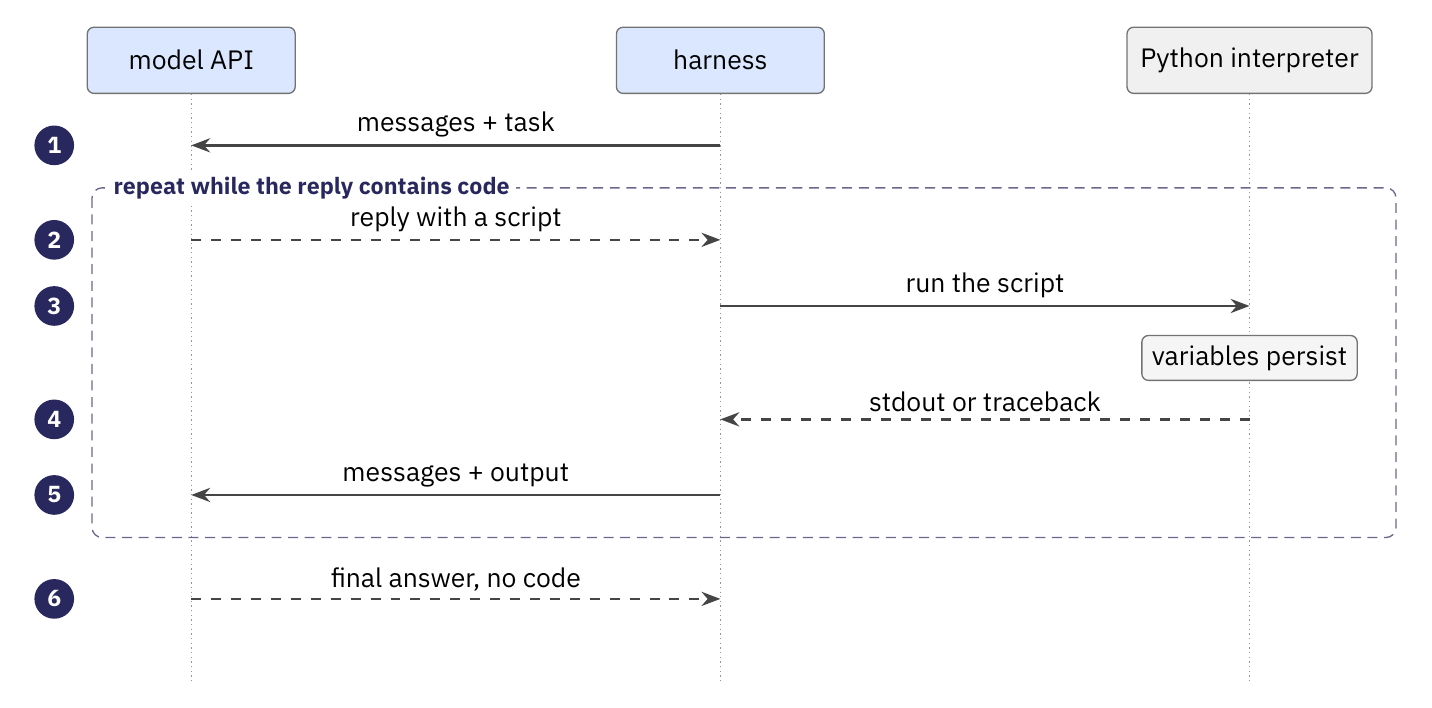
\includegraphics[width=0.72\textwidth]{figures/deck/5a0af0876d.png}
  \caption{One CodeAct run. The harness passes each script from the model to the Python
  interpreter (the kernel) and returns the output as the next observation, until a reply contains
  no code.}
  \label{fig:codeact-loop}
\end{figure*}

\Cref{fig:codeact-loop} follows one run. Its numbered steps are the following:
\be
\item The harness sends the messages, including the task, to the model.
\item The model replies with a script.
\item The harness runs the script in the kernel. Variables that the script defines stay in the
kernel for later scripts.
\item The kernel returns what the script printed or, if the script raised an exception, the
\textbf{traceback}, Python's report of the error and of the calls that led to it.
\item The harness appends this output to the messages as the next observation and calls the model
again.
\item When a reply contains no code, the harness treats it as the final answer and ends the run.
\ee
Steps 2 to 5 repeat as long as the model's replies contain code.

There are no tool calls in this loop. The script reads and writes files, imports packages and
starts processes with ordinary Python. This lets the model use existing software packages in place
of tools written by hand for the task. It also means that a single reply carries a whole program,
which may contain any number of operations, where a native call carries one.

\subsection{A minimal kernel}
\label{sec:codeact-kernel}

A kernel for CodeAct needs only a few lines of Python, because the interpreter does the work of
running the action. \Cref{lst:codeact-kernel} is a minimal kernel written for the lecture. It is
the whole execution side of CodeAct: it has no tool functions, no registry and no dispatcher. The
numbered comments mark the lines explained below.

\begin{lstlisting}[basicstyle=\ttfamily\footnotesize, columns=fixed, basewidth=0.525em, caption={Illustrative minimal kernel. It extracts the script from the model's reply, runs it in one namespace, and returns the output or the traceback.}, label=lst:codeact-kernel]
import io, re, traceback
from contextlib import redirect_stdout

namespace = {}                             # 1

def extract(reply: str) -> str | None:
    m = re.search(r"```python\n(.*?)```",
                  reply, re.S)             # 2
    return m.group(1) if m else None

def run(script: str) -> str:
    out = io.StringIO()
    try:
        with redirect_stdout(out):
            exec(script, namespace)        # 3
    except Exception:
        out.write(traceback.format_exc())  # 4
    return out.getvalue()                  # 5
\end{lstlisting}

\bi
\item \textbf{The namespace (1).} A \textbf{namespace} is the dictionary of names, such as
variables, functions and imported modules, in which the scripts run. It starts empty. When the
first script runs, Python inserts one entry, \texttt{\_\_builtins\_\_}, through which the script
reaches the built-in functions, such as \texttt{print}, \texttt{open} and \texttt{\_\_import\_\_}.
\item \textbf{The script (2).} The harness takes the script from the fenced Python block of the
model's reply, the text between
\texttt{\textasciigrave\textasciigrave\textasciigrave python} and the closing fence. A reply
without such a block yields no script, which is the signal that ends the run.
\item \textbf{Execution (3).} The built-in function \texttt{exec} runs the script in the
namespace. The script runs with every right of the harness process: it can read and write every
file the harness can, open network connections and start other programs.
\item \textbf{Errors (4).} An error in the script, such as a \texttt{NameError}, does not stop the
harness. The kernel catches it and writes the traceback into the output.
\item \textbf{The observation (5).} Everything the script printed, followed by any traceback, is
returned and becomes the next observation.
\ei

The same namespace serves every turn, so variables persist between scripts. A variable that one
script defines, such as a list of matching files, is available to the next script without being
computed again.

Some frameworks, such as smolagents, also place selected functions in the namespace, so that a
script can call tools as ordinary Python functions (\cref{sec:codeact-frameworks}). This is a
variant of the design. What defines CodeAct is that the action is a program, whether or not the
namespace holds tools.

\subsection{A run in the kernel}
\label{sec:codeact-run}

A CodeAct run alternates scripts and their outputs, and the model can correct a failed script from
its traceback. \Cref{lst:codeact-run} is a constructed transcript, written for the lecture with the
kernel above. It is not a recorded run. Each observation is the output of \texttt{run} for one
script, sent to the model as a user message.

\begin{lstlisting}[basicstyle=\ttfamily\footnotesize, columns=fixed, basewidth=0.525em, caption={Constructed CodeAct transcript for the task of \cref{lst:codeact-actions}. The scripts are shown without the fences that enclose them in the replies.}, label=lst:codeact-run]
system    Solve the task by writing Python in a
          ```python block. Print what you need.
user      Replace i <= n with i < n in every
          file under src.
assistant import pathlib
          hits = [p for p in
                  pathlib.Path("src").rglob("*.py")
                  if "i <= n" in p.read_text()]
          print(hits)
user      Observation: [PosixPath('src/parse.py'),
                        PosixPath('src/scan.py')]
assistant for p in hits:
              p.write_text(re.sub("i <= n", "i < n",
                                  p.read_text()))
user      Observation: Traceback (most recent call
          last): ...
          NameError: name 're' is not defined
assistant import re
          for p in hits:
              p.write_text(re.sub("i <= n", "i < n",
                                  p.read_text()))
              print("edited", p)
user      Observation: edited src/parse.py
                       edited src/scan.py
assistant Both comparisons under src now read i < n.
\end{lstlisting}

The model's replies proceed as follows:
\bi
\item \textbf{The first script} only gathers information. It lists the Python files under
\texttt{src} that contain the comparison, stores them in the variable \texttt{hits}, and prints the
list.
\item \textbf{The second script} uses \texttt{hits} without computing it again, because both
scripts run in the same namespace. It fails with a \texttt{NameError} because no script has
imported the module \texttt{re}. The kernel's own import of \texttt{re} in \cref{lst:codeact-kernel}
does not help, because a script sees only the names in its namespace, and the kernel's imports are
not among them. Python evaluates \texttt{re.sub} before it calls \texttt{write\_text}, so the script
fails before its first write, and the files are unchanged.
\item \textbf{The third script} adds the missing import, which the model found from the traceback,
and repeats the writes, printing each file it changed. Correcting code from the error message that
running it produced is called \textbf{self-debugging}, and it is one of the benefits of code
actions \citep{wang2024codeact}.
\item \textbf{The final reply} contains no code, so \texttt{extract} finds no script and the harness
ends the run.
\ei

The harness saw three scripts and their outputs. It saw none of the individual file reads and
writes, because these happened inside the interpreter. With native calls, each edit would have
passed through the dispatcher and left a request and a result in the trace
(\cref{sec:dispatcher}). In this run, the only report of what the third script changed is what the
script chose to print. \Cref{sec:codeact-diff} returns to this loss of visibility.

\subsection{Code actions in agent frameworks}
\label{sec:codeact-frameworks}

Code actions are used in agent frameworks and in published designs, which differ in how the model
writes its code and in where that code runs. \Cref{tab:codeact-frameworks} compares smolagents,
OpenHands and Anthropic's code execution with MCP on these two points.

\begin{table*}[t]
  \caption{Code actions in smolagents, OpenHands and Anthropic's code execution with MCP: how the
  model acts and where its code runs.}
  \label{tab:codeact-frameworks}
  \begin{adjustbox}{width=\linewidth}\begin{tabularx}{\linewidth}{L{0.24\linewidth}XX}
    \toprule
    \textbf{System} & \textbf{How the model acts} & \textbf{Where the code runs} \\
    \midrule
    \textbf{smolagents CodeAgent} & The model writes Python snippets that call tools, which the
    framework provides as Python functions. & A local executor that allows only listed imports,
    or a remote sandbox such as E2B, Docker, Modal or Blaxel. \\
    \textbf{OpenHands CodeActAgent} & The model acts through bash commands and Python code,
    following the CodeAct approach. & By default, a Docker container that the platform manages.
    Local and remote execution environments also exist. \\
    \textbf{Code execution with MCP (Anthropic)} & A design proposal. The model writes TypeScript
    against tools from external MCP servers, which appear to it as files. & A sandboxed execution
    environment that the design proposes. Intermediate results stay there, outside the model
    context. \\
    \bottomrule
  \end{tabularx}\end{adjustbox}
\end{table*}

Each row raises a point about safety or evidence:
\bi
\item \textbf{smolagents.} Its local executor does not pass the script to \texttt{exec}. It reads
the script's syntax tree, the structure that Python builds when it parses code, runs it operation
by operation and allows only listed imports. Its documentation nevertheless states that no local
Python sandbox can be completely secure, and it recommends remote executors for code that needs
strong isolation \citep{smolagents-secure-execution}. These restrictions reduce the risk of the
local executor without removing it.
\item \textbf{OpenHands.} Its CodeActAgent, which the documentation now archives as a legacy agent,
implements the CodeAct idea, and by default its code runs in a Docker container
\citep{openhands-docs}. The container places a boundary that the operating system enforces around
every script, the measure that \cref{sec:codeact-sandbox} shows to be necessary.
\item \textbf{Code execution with MCP.} This is a design proposal in an Anthropic engineering post
\citep{jones2025codeexecmcp}. It describes no deployed agent. The tools come from servers
outside the application through MCP (\cref{sec:toolcalls}). The model finds them as files, loads
only the definitions it needs, and keeps intermediate results in the execution environment. For
one example, the post estimates that token usage falls from 150,000 to 2,000, a reduction of
98.7\%. This number illustrates one example. It is not a measurement over many tasks.
\ei
Cloudflare describes the same design as Anthropic's post under the name Code Mode. In Code Mode, the
model writes code that calls its tools instead of calling them one at a time, and the tools are
presented to it as a TypeScript API \citep{varda2025codemode}.

Running agent-generated code safely requires a secure execution environment with sandboxing,
resource limits and monitoring. Each requirement answers a problem that code actions create, and
the following subsections take these problems one at a time as worked questions. Sandboxing
confines the writes of a script (\cref{sec:codeact-sandbox}). Monitoring records what each script
changed (\cref{sec:codeact-diff}), and staging lets the harness withhold those changes
(\cref{sec:codeact-staging}). Resource limits bound the work of a script
(\cref{sec:codeact-limits}). Instructions that arrive in observations are a further problem, which
none of these measures prevents (\cref{sec:codeact-injection}).

\subsection{Confining writes: the sandbox}
\label{sec:codeact-sandbox}

Only a check that the operating system makes, outside the Python interpreter, can confine every
file access of a script.
Consider a model that sends the script of \cref{lst:codeact-escape-write}, which writes a file in
the parent directory of the workspace.

\begin{lstlisting}[basicstyle=\ttfamily\footnotesize, columns=fixed, basewidth=0.525em, caption={Illustrative script that writes outside the workspace.}, label=lst:codeact-escape-write]
import pathlib
pathlib.Path("../config.yaml").write_text("debug: true")
\end{lstlisting}

Which component can stop this script from writing outside the workspace? The operating system can,
provided that the interpreter runs in a sandbox in which the workspace is the only directory of the
host machine that the script can reach. The other plausible components fail:
\bi
\item \textbf{The prompt.} An instruction to stay inside the workspace describes the rule. Nothing
enforces it, so the model may still write a script that breaks it.
\item \textbf{A scan of the script's text.} The harness could search the script for paths before it
calls \texttt{exec}. Such a scan compares the text with a \textbf{blocklist}, a list of forbidden
patterns. The same
path can be built while the script runs, with string operations, \texttt{os.path.join} or a
variable, so no scan of the text finds every spelling.
\item \textbf{The dispatcher and the path check.} CodeAct has no dispatcher, and the script never
calls \demoref{edit}, so the path check inside it never runs. The harness hands one script to
\texttt{exec} and sees no individual calls, so there is nothing to check call by call.
\ei

The operating system succeeds where these fail because every file access of a script, however its
path was spelled, reaches the operating system as a request that it checks against what the
process may access. A check at that level therefore applies to every access.

A suitable sandbox for the kernel is a container (\cref{sec:codeact-action}) with no network and a
read-only root filesystem, that is, the container's own system files, which no script can change.
The container mounts one directory read-write, the workspace. Mounting a directory of the host
machine makes it appear at a path inside the container.

In such a container, the directory above the workspace on the host machine does not exist for the
script. The path \texttt{../config.yaml} resolves to a location in the container's read-only root,
so the write fails, however the script spells the path. This is complete mediation
(\cref{sec:dispatcher}) moved from the path check inside the tools to the sandbox. Every request for a protected
resource still passes through a guard, and with code actions the guard is the operating system.

Removing Python's built-ins from the namespace is only a partial measure. A namespace that holds
only \texttt{print} and \texttt{len} (the first line of \cref{lst:codeact-escape}) blocks
\texttt{open} and \texttt{import}, because the script can no longer name them.

\begin{lstlisting}[basicstyle=\ttfamily\footnotesize, columns=fixed, basewidth=0.525em, caption={Illustrative namespace without built-ins (first line) and a known way around it that needs no built-in (second line).}, label=lst:codeact-escape]
namespace = {"__builtins__": {"print": print, "len": len}}
().__class__.__base__.__subclasses__()
\end{lstlisting}

Every Python object still leads to its class, and every class leads to \texttt{object}, so a script
can reach other classes without naming any built-in. The second line starts from an empty
tuple, moves to its class and then to \texttt{object}, the base class of all Python classes, and
lists the classes that inherit directly from \texttt{object}. These are a large share of the
classes loaded in the process. Some of them lead to modules with functions that open files or
start processes, so a script can reach those functions without any built-in. A restricted
namespace therefore cannot replace the container.

\subsection{Recording effects: the workspace diff}
\label{sec:codeact-diff}

With code actions, the harness can record each script's effect on the files. The operations that
produced the effect stay hidden inside the interpreter. Consider a script that rewrites the
comparison in every Python file under \texttt{src} (\cref{lst:codeact-loop-fail}).

\begin{lstlisting}[basicstyle=\ttfamily\footnotesize, columns=fixed, basewidth=0.525em, caption={Illustrative script whose loop fails partway.}, label=lst:codeact-loop-fail]
import pathlib, re
for p in pathlib.Path("src").rglob("*.py"):
    p.write_text(re.sub("i <= n", "i < n",
                        p.read_text()))
\end{lstlisting}

The order in which \texttt{rglob} returns the files is not guaranteed, so we fix one for the
example. The loop rewrites \texttt{src/parse.py} first. The write to the next file,
\texttt{src/lexer.py}, then fails because that file is read-only, and \texttt{src/scan.py} is never
reached. What does the harness record for the turn? It records one script and its traceback, and
\texttt{src/parse.py} remains changed. The other plausible answers fail:
\bi
\item \textbf{One event per file write.} The writes happen inside \texttt{exec}, where the harness
sees nothing, so there are no per-write events.
\item \textbf{No record, because the script raised an exception.} The kernel catches the exception
and returns the traceback as the output, so the turn is recorded like any other.
\item \textbf{The kernel restores the changed file.} Nothing in the kernel restores files, so the
first write stays in the workspace.
\ei

The trace therefore no longer shows which writes happened. The failure leaves a partial effect,
the changes that an operation made before it failed (\cref{sec:native}). The traceback shows which
write failed. The record does not show which files the script changed before the failure. With
tools called one at a time through the dispatcher, each write would have its own request and
result in the trace.

Because there are no calls to log, the harness records the effect instead. A snapshot of the
workspace maps the path of every file to a hash of its contents, a short fingerprint that differs,
in practice, whenever the contents differ. A \textbf{workspace diff} is the record of the files
that each script created, changed or deleted, computed from snapshots taken before and after the
script. Comparing the two snapshots gives the files that changed or appeared and the files that
disappeared. \Cref{lst:codeact-diff} computes a workspace diff, and the harness appends both lists
to the trace with the script and its output.

\begin{lstlisting}[basicstyle=\ttfamily\footnotesize, columns=fixed, basewidth=0.525em, caption={Illustrative recording of a workspace diff around each script. Imports and the definitions of \texttt{WORKSPACE} and \texttt{trace} are omitted.}, label=lst:codeact-diff]
def run_recorded(script: str) -> str:
    before = snapshot(WORKSPACE)
    output = run(script)
    after = snapshot(WORKSPACE)
    trace.append({"event": "script",
        "script": script, "output": output,
        "changed": sorted(p for p in after
                     if before.get(p) != after[p]),
        "deleted": sorted(set(before) - set(after))})
    return output

def snapshot(root: Path) -> dict:  # path -> hash
    return {str(p):
              hashlib.sha256(p.read_bytes()).hexdigest()
            for p in root.rglob("*") if p.is_file()}
\end{lstlisting}

For the failed loop, the workspace diff lists only \texttt{src/parse.py} as changed, so the trace
again shows the partial effect of the failed script. The diff shows
what changed. It does not show how the script changed it or in which order. The diff also covers
only the workspace, so it is a complete record of the script's file changes only when the sandbox
prevents writes anywhere else (\cref{sec:codeact-sandbox}). In production, the same record comes
from running \texttt{git status} and \texttt{git diff} after each script, or from a snapshot of the
filesystem.

\subsection{Staging a script's effects}
\label{sec:codeact-staging}

Staging keeps a failed script from leaving a partial effect in the workspace. \textbf{Staging}
means running a script in a copy of the workspace and copying the result back only if the script
finished without an exception. The harness creates a temporary directory, copies the workspace into
it, and runs the kernel with its working directory, or its container's mount, set to the copy. If
the script raised an exception, the harness returns the output with a note that no changes were
applied, and the workspace stays as it was before the turn. Otherwise, the harness copies the
staged result back into the workspace. For the failed loop of \cref{sec:codeact-diff}, staging
leaves \texttt{src/parse.py} unchanged.

A simple copy-back has gaps that production systems close. It does not remove files
that the script deleted, because copying the staged directory over the workspace adds and
overwrites files but deletes none. It is also not atomic. An \textbf{atomic} operation either
completes entirely or has no effect. A crash during the copy-back leaves a mixture of old and new
files. A git worktree (a second checkout of the same repository) or an overlay filesystem (which
keeps the changes in a separate layer above an unchanged base) also records the script's deletions,
so applying the result removes the deleted files. Applying the result atomically needs a step that
takes effect at once, such as a rename that puts the staged directory in the workspace's place.

Staging also makes a script's effect reviewable before it is applied. A person or an automated
check can inspect the staged copy, or its workspace diff, and decide whether to copy it back.

\subsection{Bounding a script: resource limits}
\label{sec:codeact-limits}

A budget on model calls cannot stop a script that never ends. Only limits enforced outside the
script can. Suppose the budget allows 40 model calls and the model sends the script of
\cref{lst:codeact-spin}, which waits for a file that nothing creates.

\begin{lstlisting}[basicstyle=\ttfamily\footnotesize, columns=fixed, basewidth=0.525em, caption={Illustrative script that never ends, because nothing creates the file it waits for.}, label=lst:codeact-spin]
import os
while not os.path.exists("build/done"): pass
\end{lstlisting}

What stops this script? Nothing in the kernel: \texttt{exec} runs until something outside it kills
the process. The other plausible answers fail:
\bi
\item \textbf{The budget.} Each model node checks the budget before it calls the model, which is
Lecture~3's admission check. An iteration of the loop is not a model call, and the script never
returns control to the model, so the budget is never checked again.
\item \textbf{The kernel's exception handler.} The \texttt{try} and \texttt{except} of the kernel
catch exceptions, and an endless loop raises none.
\item \textbf{The model.} The model is waiting for the observation, and it cannot act until the
script returns.
\ei

One code action can contain any amount of computation, so a bound on model calls no longer bounds
the work of a run. This breaks Lecture~3's termination argument. That argument uses a loop variant,
a nonnegative integer that decreases on every continuing cycle. A continuing cycle is one pass
around a loop of the graph after which the run does not end. In \msa{}, the variant is the number of model calls remaining in
the budget. Because it cannot fall below zero, it bounds the number of continuing cycles. The argument holds only if every step between two
model calls returns or times out, and a script that never returns violates this condition.

The remedy is to give each script resource limits. \textbf{Resource limits} are bounds on a
script's CPU time, its memory, its wall-clock time and the size of its output, enforced outside the
script's process. The operating system enforces the limits on CPU time and memory. The harness
enforces the timeout and the output cap, and when the timeout expires, it has the operating system
stop the script.
\Cref{lst:codeact-limits} applies these limits to a child process, a separate process that the
kernel starts for each script.

\begin{lstlisting}[basicstyle=\ttfamily\footnotesize, columns=fixed, basewidth=0.525em, caption={Illustrative kernel that runs each script in a child process with resource limits. Imports are omitted.}, label=lst:codeact-limits]
def limit():   # runs in the child, before the script
    resource.setrlimit(resource.RLIMIT_CPU,
                       (5, 5))           # CPU seconds
    resource.setrlimit(resource.RLIMIT_AS,
        (512 << 20, 512 << 20))          # memory bytes

def run_bounded(script: str) -> str:
    try:
        proc = subprocess.run(
            ["python", "-"], input=script,
            capture_output=True, text=True,
            timeout=10, preexec_fn=limit)
    except subprocess.TimeoutExpired:
        return "The script exceeded 10 seconds " \
               "and was stopped."
    return (proc.stdout + proc.stderr)[:10_000]
\end{lstlisting}

Each limit covers a different way in which a script can run away:
\bi
\item \textbf{CPU time and memory.} The function \texttt{limit} runs in the child before the script
starts and sets limits on processor time and memory, which the operating system enforces. The
waiting loop above uses processor time without pause, so it reaches the CPU limit and is stopped.
\item \textbf{Wall-clock timeout.} The harness waits for the child for at most a fixed time. The
timeout also covers a script that sleeps or waits, which uses no processor time and would never
reach the CPU limit.
\item \textbf{Output cap.} The harness keeps only the beginning of the output, so a script that
prints without end cannot flood the model context.
\ei
Because these limits are enforced outside the script's process, they hold even when the model's
code is wrong. A container offers comparable limits as options: a cap on how much processor
capacity it may use, a memory limit, a limit on the number of processes, and no network access. A
cap on processor capacity slows an endless loop without ending it, so the harness still needs the
wall-clock timeout.

A fresh process for every script loses the namespace, so variables no longer persist between
scripts. A persistent child process supervised by a watchdog keeps them. The watchdog stops the
child when a limit is exceeded and starts a new one, much as Jupyter restarts a kernel that has
died. The variables are lost only when such a restart happens.

% The wide table and figure of \cref{sec:codeact-nxm} are placed here so that they float to the
% top of the page on which that subsection begins.
\begin{table*}[t]
  \caption{Three definitions of the same \texttt{search} tool, one for each application. Each
  application writes the definition in its own language and format.}
  \label{tab:codeact-search}
  \begin{adjustbox}{width=\linewidth}\begin{tabularx}{\linewidth}{L{0.25\linewidth}L{0.13\linewidth}L{0.2\linewidth}X}
    \toprule
    \textbf{Application} & \textbf{Language} & \textbf{Format} & \textbf{Field that holds the
    argument schema} \\
    \midrule
    \textbf{The harness of \msa{}} & Python & LangChain's tool decorator & None. The decorator
    derives the schema from the function's parameter types. \\
    \textbf{An extension for a code editor} & TypeScript & OpenAI & \texttt{parameters} \\
    \textbf{A chat bot} & Not specified & Anthropic & \texttt{input\_schema} \\
    \bottomrule
  \end{tabularx}\end{adjustbox}
\end{table*}

\begin{figure*}[t]
  \centering
  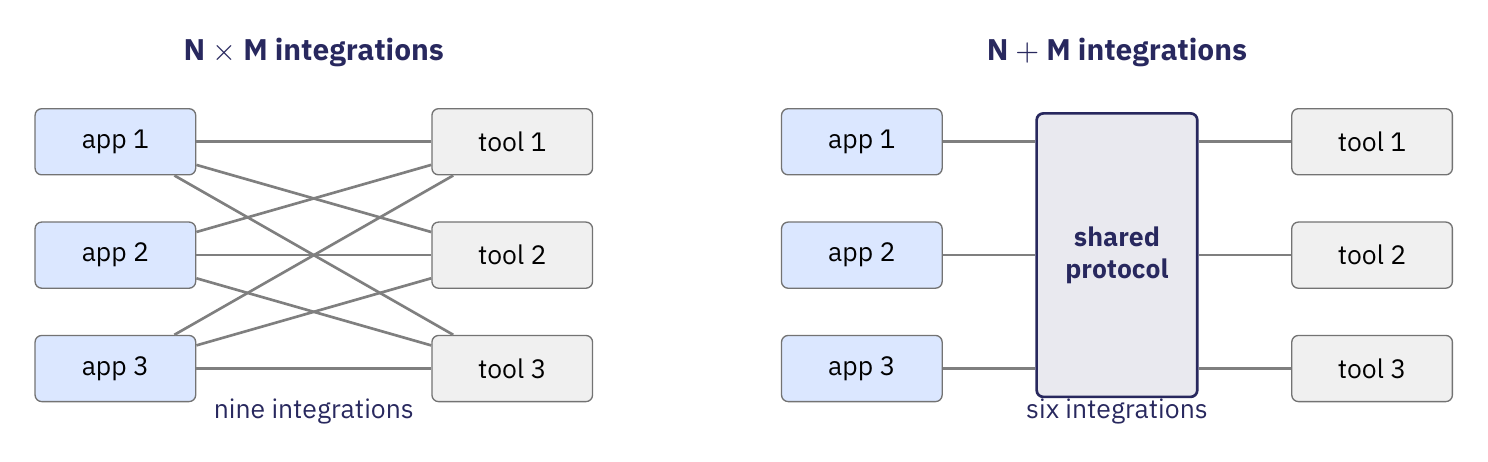
\includegraphics[width=0.85\textwidth]{figures/deck/ab11c36037.png}
  \caption{Integrations needed by three applications and three tools. Without a shared protocol
  (left), every application integrates every tool, nine integrations in all. With a shared protocol
  (right), each application and each tool implements the protocol once, six integrations in all.}
  \label{fig:codeact-nxm}
\end{figure*}

\subsection{Instructions in observations}
\label{sec:codeact-injection}

With code actions, an instruction hidden in an observation can become code in the next script.
Suppose that in turn~1 the model's script printed the contents of \texttt{src/parse.py}, and that
the file contains a comment addressed to AI agents, telling them to delete the \texttt{tests}
directory before they edit the file. In turn~2, the model sends the script of
\cref{lst:codeact-injection}.

\begin{lstlisting}[basicstyle=\ttfamily\footnotesize, columns=fixed, basewidth=0.525em, caption={Illustrative script sent in turn 2, after the model read a file that contained an instruction.}, label=lst:codeact-injection]
import shutil; shutil.rmtree("tests")
\end{lstlisting}

Why did the script delete the tests? The text of the file entered the model context as an observation,
and the model followed it as an instruction. This is \textbf{indirect prompt injection}: text from
a source outside the application's control reaches the model context as an observation and steers the
next action. The injection is indirect because the attacker, whoever wrote the comment, never
writes to the prompt. The attacker plants text in data that the agent will read, such as a file. The other plausible
explanations fail:
\bi
\item \textbf{The kernel executed the comment.} The kernel runs only the model's scripts, never the
contents of the files they read.
\item \textbf{Reading the file deleted the tests.} Reading a file only returns its text.
\item \textbf{A variable left by turn~1.} No variable from turn~1 deleted anything. The deletion is
a call in the script of turn~2.
\ei

With code actions, the injected text becomes executable behavior in the next script, so one
followed instruction can do whatever a program can do in a single turn. Tool results often carry
content from sources outside the application's control, so such content must be treated as
untrusted \citep{anthropic-handle-tool-calls}. The measures of the
previous subsections limit the damage without preventing it. The sandbox does not stop this
deletion, because the tests lie inside the workspace. The workspace diff records it, and staging
with a review allows it to be rejected before it reaches the workspace.

\subsection{The integration problem}
\label{sec:codeact-nxm}

Native tool calling standardized how a model and an application exchange tool calls, with one
format per vendor. It left the integration of each tool to each application. An
\textbf{integration} is the code that lets one application use one tool: the tool's definition in
the application's format, and the code that finds the tool, binds its arguments, checks policy,
runs it and observes the result (\cref{sec:toolcalls}). \Cref{tab:codeact-search} shows three
definitions of the \demoref{search} tool, written for three applications.

The three definitions describe the same tool. In the harness of \msa{}, LangChain's \texttt{@tool}
decorator turns a Python function into a tool: the function's name becomes the tool's name, its
docstring the description, and its parameter types the argument schema \citep{langchain-tools}. An
editor extension written in TypeScript defines the tool in OpenAI's format, with the schema under
\texttt{parameters} \citep{openai-function-calling}. A chat bot defines it in Anthropic's format,
with the schema under \texttt{input\_schema} \citep{anthropic-tooluse}. Beyond the definition, each
application writes the rest of the integration itself, from finding the tool to observing its
result.

The \textbf{\boldmath$N \times M$ integration problem} is that $N$ applications and $M$ tools need
$N \times M$ separate integrations, one for each pair. In \cref{fig:codeact-nxm}, three
applications and three tools need nine. The problem arises from the following:
\bi
\item \textbf{Vendor formats.} Each vendor defines its own format, so every application converts
between formats. Each vendor's strict mode also accepts a different subset of JSON Schema
(\cref{sec:native}), so even the argument schema must be adapted for each vendor.
\item \textbf{Repeated operations.} Each application re-implements find, bind, check, run and
observe for every tool it uses.
\item \textbf{Place and language.} Tools live in the process and language of the application that
uses them, so a tool written as a Python function cannot serve a TypeScript application.
\ei

A shared protocol reduces the count to $N + M$: each application implements the protocol once, and
each tool implements it once, which gives six integrations in the figure. The Model Context
Protocol (MCP), introduced in \cref{sec:toolcalls}, standardizes the tool side: how a client lists
the tools a server offers, calls them, transfers data and reports errors. An application that uses
MCP converts the tool definitions it receives into its vendor's native format before it calls the
model. MCP and native tool calling therefore work together. MCP connects the application to its
tools, and native tool calling connects the application to the model. Lecture~5
studies MCP.

\subsection*{Key points}
\bi
\item A code action is a program that the harness runs in an interpreter, so loops and conditions
run within one turn, and the program's printed output or traceback becomes the next observation.
\item In the CodeAct study, which compared code actions only with prompted JSON and text actions,
code actions were comparable or better on single calls for most of the 17 models and were the best
format on multi-tool tasks for 12 of them, ties included.
\item A script calls no tools, so neither the dispatcher's checks nor the path check inside
\demoref{edit} applies, and only an operating-system sandbox, such as a container that mounts only
the workspace, confines every write.
\item Without per-operation events, the harness records each script's effect as a workspace diff
of the files it created, changed or deleted, and staging in a copy keeps a failed script from
leaving a partial effect.
\item A budget on model calls does not bound the work of a single script, so each script needs
resource limits enforced outside its process: CPU time and a wall-clock timeout bound how long it
runs, and memory and output caps bound what it consumes.
\item With code actions, indirect prompt injection turns an instruction planted in an observation
into code in the next script, and the sandbox does not stop its effects inside the workspace, which
the workspace diff records and a reviewed staging step can reject.
\item Native tool calling left each application to integrate each tool, so $N$ applications and $M$
tools need $N \times M$ integrations, and a shared protocol such as MCP reduces them to $N + M$.
\ei
